\ylDisplay{Kujutis} % Ülesande nimi
{Tundmatu autor} % Autor
{piirkonnavoor} % Voor
{2013} % Aasta
{P 18} % Ülesande nr.
{3} % Raskustase
{
% Teema: Valgusõpetus
\ifStatement
Konstrueerige ruudu $ABCD$ kujutis kumerläätsega.
\begin{center}
	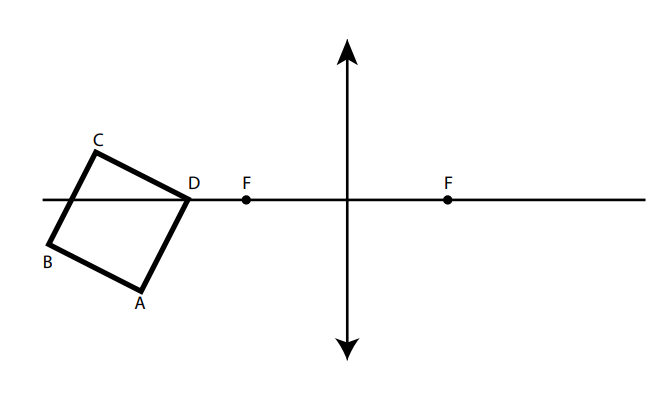
\includegraphics[width=0.5\linewidth]{2013-v2p-18-yl.PNG}
\end{center}
\fi
\ifHint
Kõige keerulisem on määrata punkti $D$ kujutise kaugust teisel pool läätse, sest see asub optilisel peateljel. Selleks võib võtta punktist $D$ optilise peateljega ühe ristsirge ning konstrueerida sellelt sirgelt mõne abipunkti kujutis teisele poole. Abipunkti kujutis peab olema samuti samal ristsirgel punkti $D$ kujutisega
\fi
\ifSolution
\begin{center}
	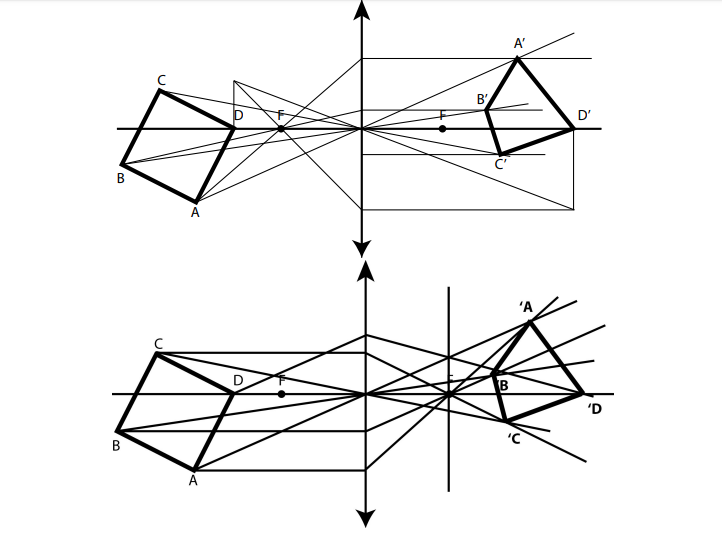
\includegraphics[width=0.5\linewidth]{2013-v2p-18-lah.PNG}
\end{center}
\fi
}